

\documentclass{article}
\usepackage[utf8]{inputenc}
\usepackage[utf8]{inputenc}
\usepackage[T1]{fontenc}
\usepackage[english]{babel}
\usepackage{fullpage}
\usepackage{color}
\usepackage[table]{xcolor}
\usepackage{listings}
 
\definecolor{darkWhite}{rgb}{0.94,0.94,0.94}
 
\lstset{
  aboveskip=3mm,
  belowskip=-2mm,
  backgroundcolor=\color{darkWhite},
  basicstyle=\footnotesize,
  breakatwhitespace=false,
  breaklines=true,
  captionpos=b,
  commentstyle=\color{red},
  deletekeywords={...},
  escapeinside={\%*}{*)},
  extendedchars=true,
  framexleftmargin=16pt,
  framextopmargin=3pt,
  framexbottommargin=6pt,
  frame=tb,
  keepspaces=true,
  keywordstyle=\color{blue},
  language=C,
  literate=
  {²}{{\textsuperscript{2}}}1
  {⁴}{{\textsuperscript{4}}}1
  {⁶}{{\textsuperscript{6}}}1
  {⁸}{{\textsuperscript{8}}}1
  {€}{{\euro{}}}1
  {é}{{\'e}}1
  {è}{{\`{e}}}1
  {ê}{{\^{e}}}1
  {ë}{{\¨{e}}}1
  {É}{{\'{E}}}1
  {Ê}{{\^{E}}}1
  {û}{{\^{u}}}1
  {ù}{{\`{u}}}1
  {â}{{\^{a}}}1
  {à}{{\`{a}}}1
  {á}{{\'{a}}}1
  {ã}{{\~{a}}}1
  {Á}{{\'{A}}}1
  {Â}{{\^{A}}}1
  {Ã}{{\~{A}}}1
  {ç}{{\c{c}}}1
  {Ç}{{\c{C}}}1
  {õ}{{\~{o}}}1
  {ó}{{\'{o}}}1
  {ô}{{\^{o}}}1
  {Õ}{{\~{O}}}1
  {Ó}{{\'{O}}}1
  {Ô}{{\^{O}}}1
  {î}{{\^{i}}}1
  {Î}{{\^{I}}}1
  {í}{{\'{i}}}1
  {Í}{{\~{Í}}}1,
  morekeywords={*,...},
  numbers=left,
  numbersep=10pt,
  numberstyle=\tiny\color{black},
  rulecolor=\color{black},
  showspaces=false,
  showstringspaces=false,
  showtabs=false,
  stepnumber=1,
  stringstyle=\color{gray},
  tabsize=4,
  title=\lstname,
}
\usepackage{graphicx}
\title{HAI804I – Codage et compression multimédia
}
\author{Fabien Caballero}

\begin{document}

\maketitle
    \tableofcontents

\newpage

\begin{figure}[h]
\centerline{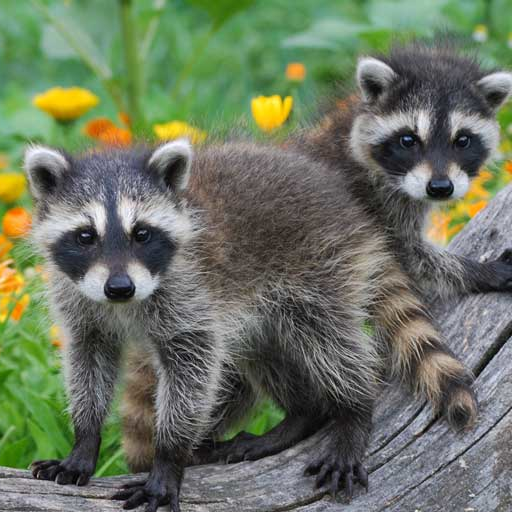
\includegraphics[scale=0.3]{./rendus/Nicoon.png}}
\caption{Image d'origine utilisée tout le long du TP}
\end{figure}

\addcontentsline{toc}{section}{Introduction}
\section*{Introduction}
Le but de ce tp est de réduire le nombre de couleurs pour réduire la taille de l'image.
On va pour cela utiliser une palette de couleur et définir la valeur d'un pixel par l'index de la couleur qu'il doit prendre dans la palette.
\\\\
\section{Algorithme K-Mean }
Pour commencer, on choisit 2 pixels de manière aléatoire, puis on y applique notre algorithme kmean.
Celui-ci se réalise en 3 étapes, la première est pour chaque pixel calculer sa distance chaque centroïds et retenir le centroïds ayant la plus petite distance avec le pixel courant.
Ainsi tout nos pixels appartiennent à une classe.
La seconde étape est de pour chaque classe faire la moyenne de tout les pixels appartenant à cette classe;
On obtient donc pour chaque classe une nouvelle valeur de centroïds.
et la troisière et dernière étape est de boucler récursivement si le pourcentage de pixels ayant changé de classe est inférieur à 10\%.

On obtient à la fin de cet algorithme un ensemble de K classes avec des centroïds offrant une classification des pixels stable.
\newpage
\section{Classification 2-mean d'une image ppm}

\begin{figure}[h]
\centerline{
\includegraphics[scale=50]{./rendus/Palette2Before.png}}
\caption{Palette des couleurs des centroïds choisis avant 2-Mean}
\end{figure}

En appliquant cet algorithme sur 2 classes avec la palette précédente on obtient, en fin d'algorithme la suivante.


\begin{figure}[h]
\centerline{
\includegraphics[scale=50]{./rendus/Palette2.png}}
\caption{Palette des couleurs des centroïds choisis avant 2-Mean}
\end{figure}


Puis en remplaçant la couleur de chaque pixel par la couleur du centroid de la classe auquel il appartient on obtient, l'image suivante.

\begin{figure}[h]
\centerline{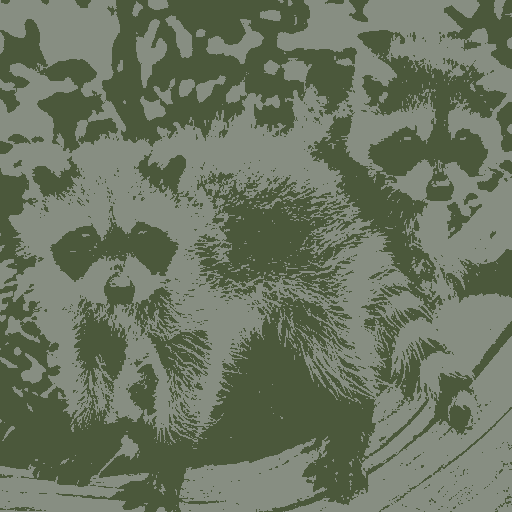
\includegraphics[scale=0.5]{./rendus/Nicoon2Color.png}}
\caption{Image résultant du 2-mean}
\end{figure}

On remarque que 2 couleurs ont étaient dominantes dans la convergence des 2 centroïds, celles-ci étant le marron et le vert car il y a une majorité de vert avec l'herbe en fond et de marron ou gris avec le tronc et les ratons-laveurs.


\section{Variation de l'image selon le nombre de classes}

\begin{figure}[h]
\centerline{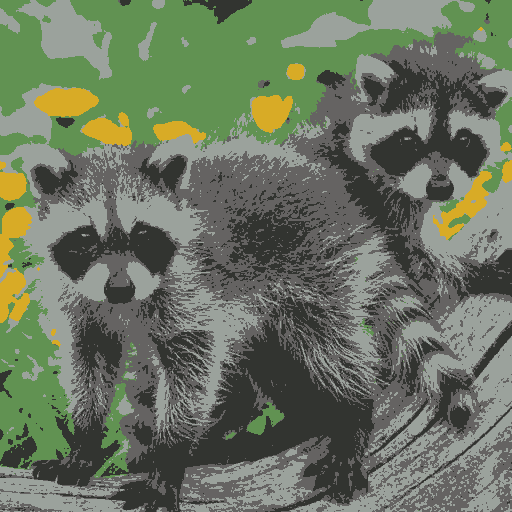
\includegraphics[scale=0.4]{./rendus/Nicoon5Color.png} 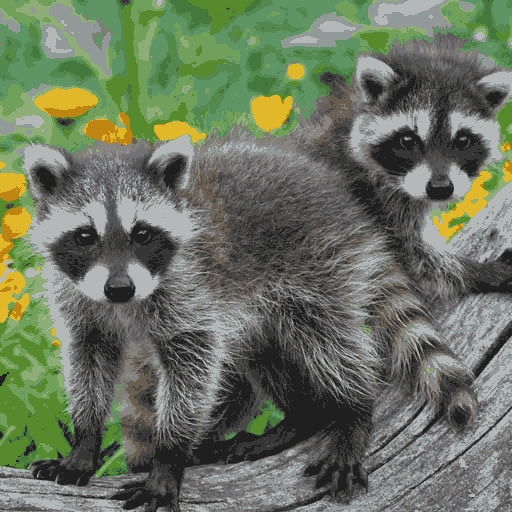
\includegraphics[scale=0.4]{./rendus/Nicoon20Color.png} 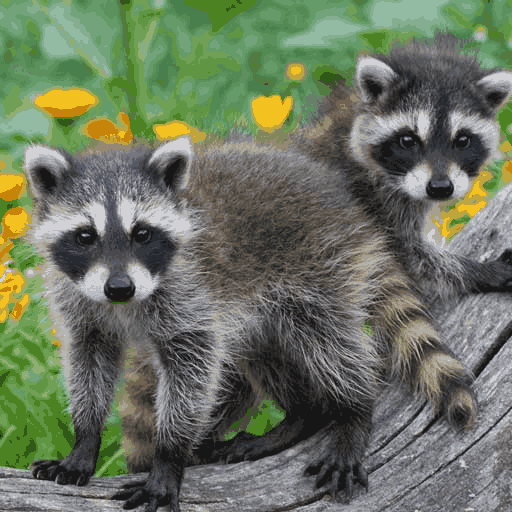
\includegraphics[scale=0.4]{./rendus/Nicoon50Color.png}}
\caption{Image résultant du 5-mean, 20-mean et 50-mean}
\end{figure}

On remarque que l'on se rapproche de l'image d'origine plus on augmente le nombre de classes, cela est dû au fait qu'il y a plus de possibilités de couleurs et donc une meilleure précision pour cibler une couleur particulière, qui a vu d'oeil semble être la même sur toute une zone lors de la classification.

\newpage
\section{Classification 256-mean d'une image ppm}

\begin{figure}[h]
\centerline{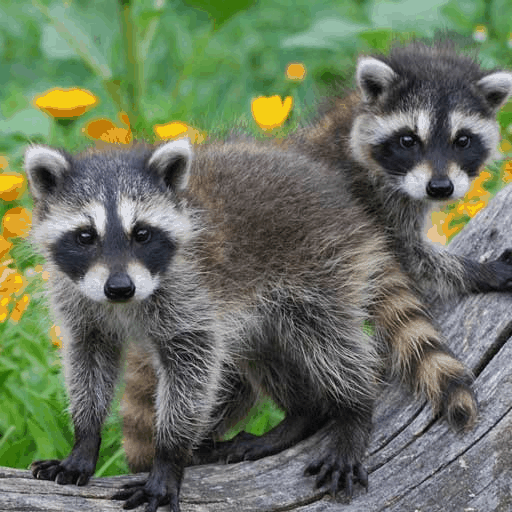
\includegraphics[scale=0.5]{./rendus/Nicoon256Color.png} 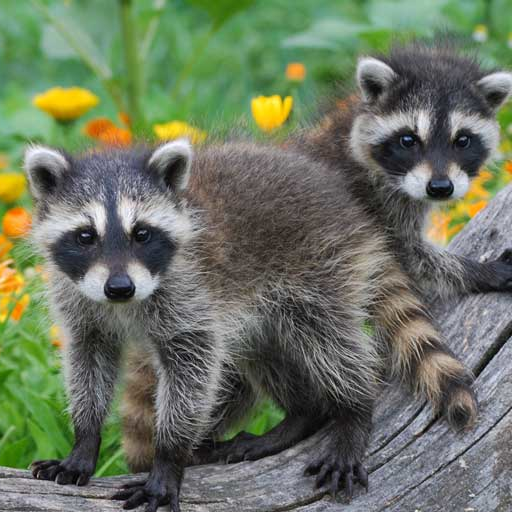
\includegraphics[scale=0.5]{./rendus/Nicoon.png}}
\caption{Image résultant du 256-mean (gauche) image originale (droite)}
\end{figure}

L'image avec 256 classes est très fidèle à celle d'origine, la différence se voit seulement sur les fleurs en fond, par exemple, car les variantes de jaune étant en minorité par rapport à celles de vert, de marron ou de gris n'ont pas eu assez d'impact sur le résultat pour pouvoir approcher l'image d'origine.

Pour mesurer le bruit entre les 2 images, on calcule le PSNR en utilisant la moyenne quadratique.
Pour l'exemple ci-dessus, on obtient donc un \textbf{PSNR de 34.1252 dB}.


\newpage
\section{Réduction de la taille de l'image}
Le fait d'avoir fait tout cela ne nous apporte rien en gain de taille d'image car chaque pixel reste malgré tout codé sur 3 octets et il y a beaucoup de répétition.
Pour réduire la taille de l'image on utilise une image composée des index correspondant à une couleur associée dans la palette de couleurs contenant toutes les couleurs des centroïds.

On obtient une image en nuance de gris et une palette de couleurs et on peut à partir de ça recréer notre image et avoir une taille approximativement divisée par 3.
Car on a maintenant seulement 1 octet par pixel et la palette à stocker donc 256*3 octets ce qui est négligeable pour de grandes images.

\begin{figure}[h]
\centerline{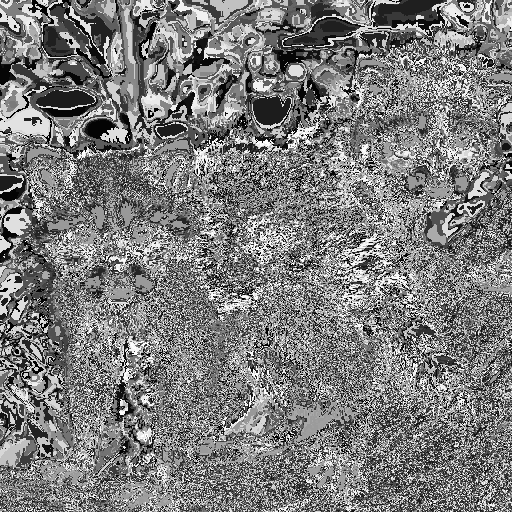
\includegraphics[scale=0.5]{./rendus/Q8.png} 
\includegraphics[scale=10]{./rendus/Palette256.png}}
\caption{Image d'index et sa base de couleurs associée (couleurs classées dans l'odre croisant de l'index)}
\end{figure}

\addcontentsline{toc}{section}{Conclusion}
\section*{Conclusion}
Ce Tp m'a permis d'approfondir la manipulation d'une image, de répondre à une problématique réelle de stockage et mettre en oeuvre une solution de compression sans trop de perdre d'informations.
La réflexion derrière le concept de classification et d'indexation de l'image était très intéressant, et permet d'essayer de voir les images et les pixels qui la composent d'une manière différente. En effet lors de la classification nos pixels peuvent très facilement vus comme un ou des nuages de points dans l'espace et notre image vue comme une tableau d'index.
J'ai trouvé très interessant ce détachement du concept classique que l'on peut avoir d'une image.

\end{document}